% This document must be compiled with LuaLaTeX
\documentclass[12pt,article]{memoir}

\usepackage[letterpaper, portrait, margin=1in]{geometry}	% Standard page setup
\usepackage[USenglish]{babel}								% English typsetting conventions
\usepackage{fancyhdr}										% Headers and footers
\usepackage{graphicx}										% Additional graphics options
\usepackage{xcolor}											% Better colors
\usepackage{xpatch}											% Better macro patches
\usepackage{hyperref}										% Hyperlinks
\usepackage{fontspec}										% Custom fonts
\usepackage{tikz}											% Graphics creation
\usepackage{float}											% Figure positioning
\usepackage{tabu}											% Better tables
\usepackage[style=ieee, backend=biber]{biblatex}			% Bibliography
\usepackage[font={small,it}]{caption}						% Italic captions
\setsansfont{NeueHaasUnicaPro}
\usetikzlibrary{calc}
\usepackage[yyyymmdd]{datetime} % change date format to yyyy/mm/dd to fit ISO8601

\renewcommand{\familydefault}{\sfdefault} % set font
\renewcommand{\dateseparator}{--} % change date-seperators to - to fit ISO8601

\renewcommand\contentsname{Table of Contents}

\chapterstyle{section}
\renewcommand*{\chapnumfont}{\normalfont\HUGE\bfseries\sffamily}
\renewcommand*{\chaptitlefont}{\normalfont\HUGE\bfseries\sffamily}

\makeatletter 
% define macro for itemcode
\newcommand\itemcode[1]{\renewcommand\@itemcode{#1}}
\newcommand\@itemcode{}

% define macro for rev number
\newcommand\revnumber[1]{\renewcommand\@revnumber{#1}}
\newcommand\@revnumber{}
\makeatother

\definecolor{orbitOrange}{RGB}{250,62,0} % the ORBiT orange

\setlrmarginsandblock{2.5cm}{2.5cm}{*}
\setulmarginsandblock{2.5cm}{*}{1}
\checkandfixthelayout 

\setlength{\beforechapskip}{0cm} % reduce chapter spacing

\hypersetup{
    colorlinks,
    citecolor=black,
    filecolor=black,
    linkcolor=black,
    urlcolor=black
}

% Background swoosh
\newcommand\OrbitBackground[1]{% For a logo drawn with TikZ
	\begin{tikzpicture}[remember picture,overlay] % draw background
	\coordinate (bl) at (current page.south west);
	\coordinate (r) at (current page.east);
	\coordinate (A) at ($(bl)+(0,3cm)$);
	\coordinate (B) at ($(r)+(0,-2cm)$);
	\coordinate (C) at (current page.south east);
	\coordinate (ctrlNode) at ($(current page.south) + (0cm,1cm)$);
	\coordinate (ctrlNode2) at ($(current page.south east) + (-1cm,1cm)$);
	\fill[orbitOrange, fill opacity={#1}]
	(A) .. controls (ctrlNode) and (ctrlNode2) .. (B) -- (C) -- (bl);
	\node [white] at ($(C) + (-3cm,1cm)$) {2015-\the\year \ ORBiT@SU};
	\end{tikzpicture}
}


%**********************************************************************
%Document titles etc. defined here: (replace [] as well)
\title{OA-II VEH COM System Design}
\author{Jinzhi Cai}
\itemcode{DR00003}
\revnumber{A02}
\date{\today}
%end of document titles etc.
%**********************************************************************

% set header style
\makeatletter
\pagestyle{fancy}
{
	\fancyheadoffset{0cm}

	\lhead{\@title \ - \@itemcode}
	\rhead{Page: \thepage }
	%\chead{\leftmark} % section name
}
\makeatother

\cfoot{\OrbitBackground{0.2}}

\begin{document}
	
\OrbitBackground{1}

\makeatletter

\includegraphics[width=\textwidth]{../Templates/logo.jpg}\\[4ex]
\begin{center}
	\bfseries \fontsize{50}{50}\selectfont  \@title \\[2ex]
	\LARGE  \@itemcode
\end{center}
\vfill
\begin{flushright}
	\LARGE Rev: \@revnumber\\
	\large \@author\\
	\large \@date\\[18ex]
\end{flushright}
\makeatother
\thispagestyle{empty}
\newpage

\tableofcontents*
\thispagestyle{fancy}
\newpage

\tableofcontents*
\clearpage


%**********************************************************************
% Everything after this is the main document. Edit below this line,

\chapter{Introduction}
\section{Scope}
This document outlines the design for the OA-II VEG Computing and Operation Module.
\section{Purpose}
The design goal is to build a system that allows real time operation and multimedia processing simultaneously during flight.
\chapter{Revision History}
\begin{table}[H]
	\centering
	\resizebox{0.8\textwidth}{!}{%
		\begin{tabu}{r || c | c | c }
		Rev\# & Editor & Delta & Date\\ \hline
		A01 & Jinzhi Cai & Initialize & 2019-7-20\\
		\end{tabu}
	}
	\caption{Summary of Revision History}
	\label{tab:rev}
\end{table}
\newpage
\chapter{Requirement Analysis}
\section{Failure Recovery}
In the OA-OII VEH requirements, failure recovery is the most critical component. Proper recovery and redundancy requires the following:

\subparagraph{Backup}Each mission critical system must have at least one backup unit.
\subparagraph{Fast Switch} When an emergency scenario is detected, the system switches to backup unit quickly, and is able to keep that system operating.
\subparagraph{Hierarchy Failure Recovery System} For each failure scenario, the recovery system has a plan to protect the device and preserve data.
\section{Realtime Operating System}
In the OA-II VEH requirements, a realtime operating system is key to performing critical procedures.
\subparagraph{Predictable Execution Time}Each operation needs to be completed within a limited time and with minimal errors.
\subparagraph{Interface with the Main System}The RTOS needs to be able to receive commands from other systems.
\subparagraph{Execution Feedback}When a procedure is completed, it will need confirmation from sensor data.
%\section{Additional Sensor Fusion}
\newpage
\chapter{Current Controller Analysis}
\section{Arduino}
Aruino is a common and beginner friendly microcontroller used in DIY electronics, and has abundant libraries for different IC. However, most of these libraries are inefficient and the interface options are limited. Its core clock runs at 16MHz which is not fast enough to support a functional Linux system.
\section{STM32 Serise}
SYM32 Series is another common microcontroller that supports up to 400MHz core clock, and also supports Linux operating systems. However, like the Arduino, it lacks support for a custom interface.
\section{Market SoC System}
SoC systems such as the Raspberry Pi and BeagleBone have a variety of interface options, but whose interfaces lack the high speed required for connections between systems.
\section{FPGA Soft Core Processor}
A field-programmable gate array (FPGA) is an integrated circuit designed to be configured by a customer or a designer after manufacturing – hence the term "field-programmable".\cite{Cite Needed} Almost every FPGA company will have it own soft core processor. This allows the core to be easily reprogrammed, as it is formed by "logical synthesis" and allow the user to rebuild them in the FPGA chip as long as the chip has enough resources. Even the soft core processor allow user to customize the structure, but the speed of soft core processor will not as fast as the SoC processor. Although, it is fairly easy to interface to other systems.
\section{SoC FPGA}
The SoC FPGA is another kind of FPGA. The difference is the embedded, more powerful processor as know as hard core processor. It helps fuse the benefit between the SoC chip and FPGA chip designs. On one hand, it allows a big system to run in the powerful hard core processor, and, at the same time, the flexibility of an FPGA chip allows a custom interface and upgradibility. However, SoC FPGAs have less logical resources compared with a classic FPGA and weak proessing power when compared with SoC which is the same cost.
\newpage
\chapter{Recommended System Design}
\section{SoC FPGA}
In this design, the main processor will be a SoC FPGA that have about 70K LUT logic resources and a dual core 800MHz - 1GHz hard core processor.
\begin{table}[H]
	\centering
	\resizebox{0.5\textwidth}{!}{%
		\begin{tabu}{ c | c }
		IP core or Logic & Resource Cost\\ \hline
		Blackbone Bus Controller & 50K(Max)\\
		Low Speed Sensor Controller & 10K\\
		Soft Core Processor & 9K\\
		Debug JTAG Core & 1K\\ \hline
		Summery & 70K
		\end{tabu}
	}
	\caption{Table of Logic Resource}
	\label{tab:rev}
\end{table}
The hard core processor will be collecting data from the bus and sensor controller. It will store that data and use it to resolve the rocket attitude and location. The result will then transfer to command and be sent to the realtime soft core processor to control the PAM.\\
The FRU will have the same hardware structure as the MCU, but constantly get data from the MCU for error checking.
\begin{center}
\begin{figure}[htp]
\begin{center}
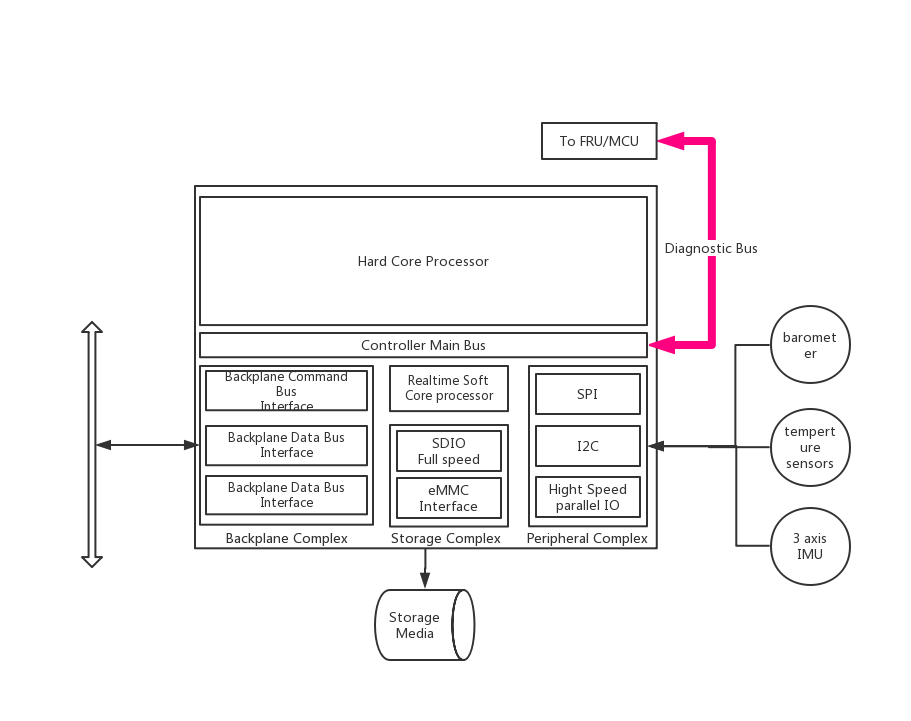
\includegraphics[width=0.6\textwidth]{img/DR00003_Plan1.png}
 \caption{Block Diagram For COM System}	
\end{center}
\end{figure}
\end{center}

%end of document
%**********************************************************************
\end{document}
